\documentclass[12pt]{article}
\usepackage{amsmath}
\usepackage{amssymb}
\usepackage{geometry}
\usepackage{enumerate}
\usepackage{natbib}
\usepackage{float}%稳定图片位置
\usepackage{graphicx}%画图
\usepackage[english]{babel}
\usepackage{a4wide}
\usepackage{indentfirst}%缩进
\usepackage{enumerate}%加序号
\usepackage{mathabx}%积分
\usepackage{multirow}%合并行
\title{\large UM-SJTU JOINT INSTITUTE\\Intro to Circuits\\(VE215)\\\ \\\ \\\ \\\ \\\ \\\ \\\ \\\ \\\ \\\ \\\
LABORATORY REPORT\\\ \\\ EXERCISE 5\\\ Filter Lab \\\ \\\ \\\ \\\ \\\ }
\author{Name: Pan Chongdan\\ID: 516370910121}
\date{Date: \today}
\begin{document}
\maketitle
\newpage
\section{Introduction and Theoretical Background}
\subsection{Objectives}
\begin{enumerate}
\item Learn about four types of filters – Low-Pass, High-Pass, Band-Pass, and Band-reject.
\item Learn about transfer functions.
\item Predict the theoretical result and make comparison with lab data.
\end{enumerate}
\subsection{Theoretical Background}
\subsubsection{Filters}
Filters are everywhere in our lives. The circuits built to operate on signals usually apply filters. For example, telephone lines pass the sounds at frequencies between about 100Hz and 3kHz and practically blocks all other frequencies.
\subsubsection{Transfer Function}
Mathematically, the transfer function is used to analyze what the circuit did to the signal:
$$Transfer Function=\frac{Output Signal}{Input Signal}$$
The function can also be expressed as 
$$H(\omega)=\frac{V_{out}(\omega)}{V_{in}(\omega)}$$
The magnitude of the transfer function is called “voltage gain”, often measured as the ratio of the peak-to-peak (ppk) voltages:
$$|H(\omega)|=|\frac{V_{out}(\omega)}{V_{in}(\omega)}|=\frac{V_{Outppk(\omega)}}{V_{Inppk}(\omega)}$$
It is convenient to express and plot the magnitude of the transfer function on the logarithmic scale using decibels:
$$|H(\omega)|_{dB}=20\cdot log_{10}\frac{V_{Outppk(\omega)}}{V_{Inppk}(\omega)}$$
Since both ppk voltages are always positive, the transfer function magnitude is positive and thus can always be converted to decibels. The use of decibels allows us to review data over a broad range.
\begin{figure}[H]
\centering
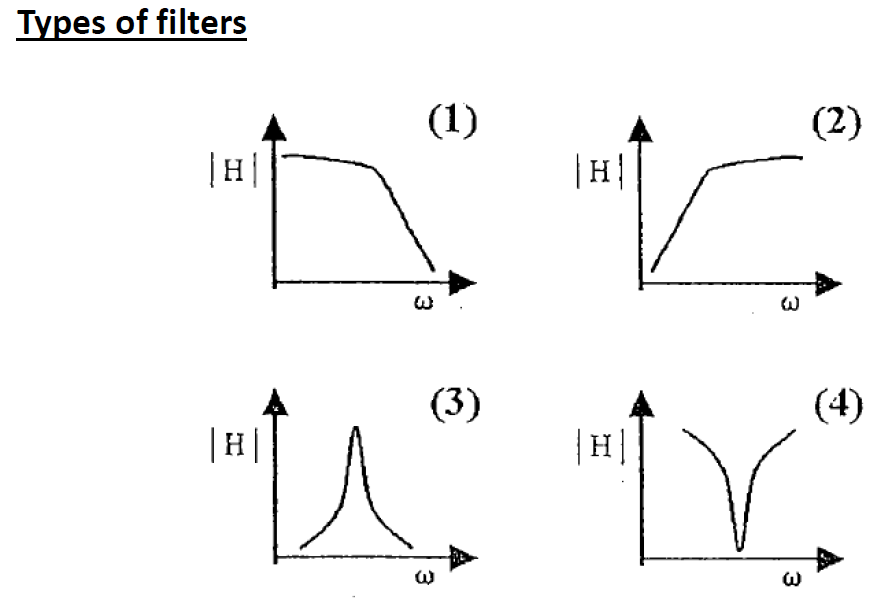
\includegraphics[scale=0.5]{P1.jpg}
\end{figure}
\par In the figure above are the four main families of filters:
\par (1): Low-Pass; (2): High-Pass; (3): Band-Pass; (4): Band-reject
\begin{figure}[H]
\centering
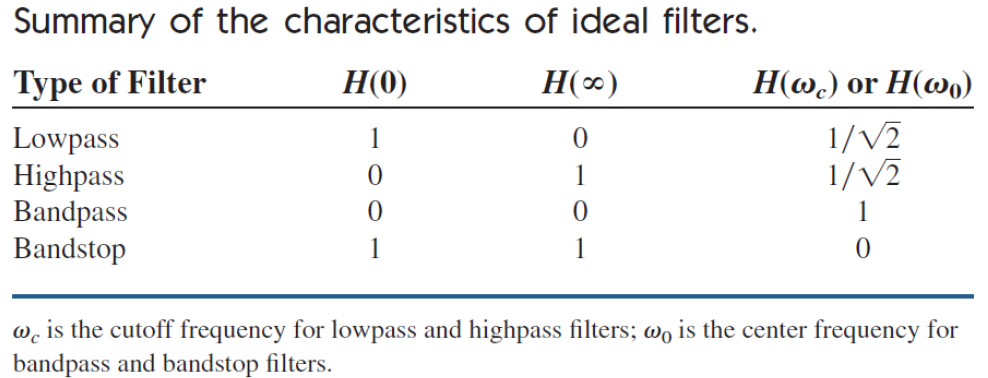
\includegraphics[scale=0.5]{P2.jpg}
\end{figure}
Filter circuits, which you are going to build in this lab, contain resistors, capacitors, and inductors. They are all passive filters.
\subsubsection{High-Pass Filter}
The high-pass filter we are going to build uses a capacitor and a resistor.
\begin{figure}[H]
\centering
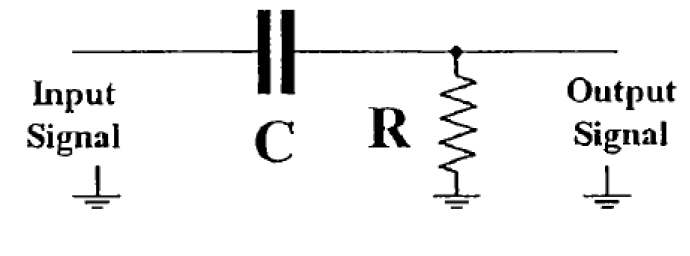
\includegraphics[scale=0.5]{P3.jpg}
\end{figure}
For the high-pass filter:
$$H(\omega)=\frac{V_{out}(\omega)}{V_{in}(\omega)}=\frac{R}{R+\frac{1}{j\omega C}}=\frac{j\omega RC}{1+j\omega RC}$$
Note that H(0)=0,H($\infty$)=1.Hence, it would only let high frequency pass.
\subsubsection{Low-Pass Filter}
The low-pass filter we are going to build uses a capacitor and a resistor.
\begin{figure}[H]
\centering
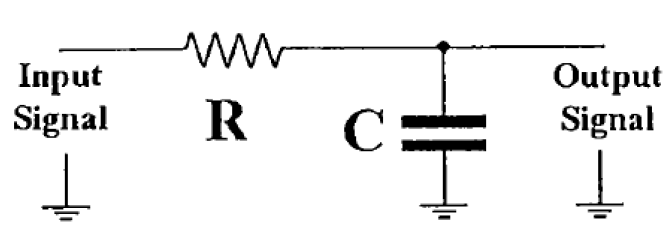
\includegraphics[scale=0.5]{P4.jpg}
\end{figure}
For the low-pass filter:
$$H(\omega)=\frac{V_{out}(\omega)}{V_{in}(\omega)}=\frac{\frac{1}{j\omega C}}{R+\frac{1}{j\omega C}}=\frac{1}{1+j\omega RC}$$
Note that H(0)=1,H($\infty$)=0.Hence, it would only let low frequency pass.
\subsubsection{Band-Pass Filter}
The band-pass filter we are going to build uses a capacitor, an inductor and a resistor.
\begin{figure}[H]
\centering
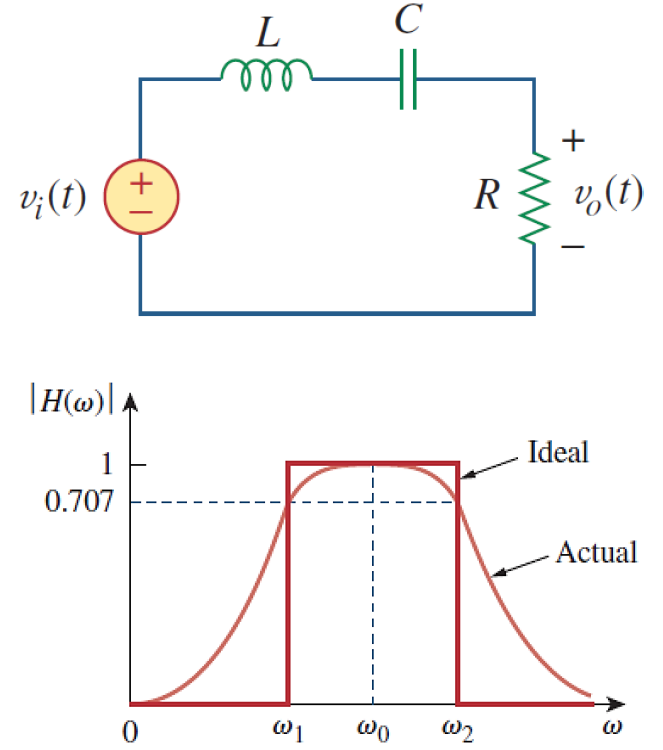
\includegraphics[scale=0.5]{P5.jpg}
\end{figure}
For the band-pass filter:
$$H(\omega)=\frac{V_{out}(\omega)}{V_{in}(\omega)}=\frac{R}{R+j(\omega L-\frac{1}{\omega C})}$$
Note that H(0)=0, H($\infty$)=0. The band-pass filter passes a band of frequencies centered on the center frequency $\omega_0$, which is given by $\omega_0=\frac{1}{\sqrt{LC}}$.
\subsubsection{Band-Stop Filter}
The band-stop filter we are going to build uses a capacitor, an inductor and a resistor.
\begin{figure}[H]
\centering
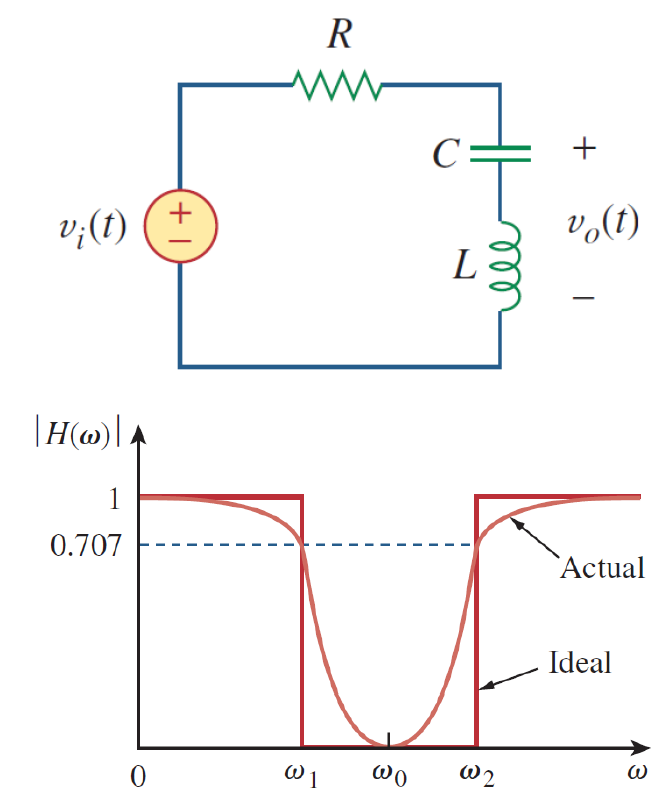
\includegraphics[scale=0.5]{P6.jpg}
\end{figure}
For the band-reject filter:
$$H(\omega)=\frac{V_{out}(\omega)}{V_{in}(\omega)}=\frac{j(\omega L-\frac{1}{\omega C})}{R+j(\omega L-\frac{1}{\omega C})}$$
Note that H(0)=0, H($\infty$)=0. The band-stop filter rejects a band of frequencies centered on the center frequency $\omega_0$, which is given by $\omega_0=\frac{1}{\sqrt{LC}}$.
\section{Procedures}
\begin{enumerate}
\item I filled the expected data column according to the pre-lab assignments.
\item I constructed the circuit for each type of filter. Resister: $R=982\Omega$;Capacitor:$C=0.1\mu F$;Inductor:$L=1mH$.
\item I set the Input Signal in the function generator to be Sine Wave with amplitude of 5 $V_{ppk}$ and changed the frequency accordingly.
\item I used the oscilloscope to detect the amplitudes of the Input and Output signals and recorded them respectively in the first two column in the tables.
\item For the band-reject filter, when the frequency approached the critical frequency at which the Transfer Function Magnitude reached its minimum, the Output Signal Amplitude was changing rapidly.
\item I calculated with the experimental data for the “Transfer function magnitude” and “Transfer function magnitude, in dB” columns.
\end{enumerate}
\section{Results}
\subsection{Low-pass Filter}
\begin{table}[H]
\centering
\begin{tabular}{|c|c|c|c|c|c|c|}
\hline
Frequency & \begin{tabular}[c]{@{}c@{}}Input signal\\ amplitude\\ $V_{\mathrm{ppk}}$\end{tabular} & \begin{tabular}[c]{@{}c@{}}Output\\ signal\\ amplitude,\\ $V_{\mathrm{ppk}}$\end{tabular} & \begin{tabular}[c]{@{}c@{}}Transfer\\ function\\ magnitude\end{tabular} & \begin{tabular}[c]{@{}c@{}}\textbf{Expected} \\ transfer\\ function\\ magnitude\end{tabular} & \begin{tabular}[c]{@{}c@{}}Transfer\\ function\\ magnitude\\ in dB\end{tabular} & \begin{tabular}[c]{@{}c@{}}\textbf{Expected}\\ transfer\\ function\\ magnitude,\\ in dB\end{tabular} \\ \hline
1MHz      & 4.78                                                                 & 0.0197                                                                      & 0.0041                                                                  & 0.0016                                                                              & -47.7443                                                                        & -55.8085                                                                                    \\ \hline
100kHz    & 4.82                                                                 & 0.114                                                                       & 0.0237                                                                  & 0.0162                                                                              & -35.8097                                                                        & -35.8070                                                                                    \\ \hline
50kHz     & 4.82                                                                 & 0.213                                                                       & 0.0442                                                                  & 0.0324                                                                              & -29.7891                                                                        & -29.7898                                                                                    \\ \hline
10kHz     & 4.86                                                                 & 0.92                                                                        & 0.1893                                                                  & 0.1600                                                                              & -15.9176                                                                        & -15.9184                                                                                    \\ \hline
5kHz      & 4.86                                                                 & 1.65                                                                        & 0.3395                                                                  & 0.3083                                                                              & -10.2205                                                                        & -10.2191                                                                                    \\ \hline
1kHz      & 5.03                                                                 & 4.14                                                                        & 0.8231                                                                  & 0.8510                                                                              & -1.4014                                                                         & -1.4010                                                                                     \\ \hline
500Hz     & 5.07                                                                 & 4.78                                                                        & 0.9428                                                                  & 0.9556                                                                              & -0.3948                                                                         & -0.3948                                                                                     \\ \hline
\end{tabular}
\end{table}
\subsection{High-pass Filter}
\begin{table}[H]
\centering
\begin{tabular}{|c|c|c|c|c|c|c|}
\hline
Frequency & \begin{tabular}[c]{@{}c@{}}Input signal\\ amplitude\\ $V_{\mathrm{ppk}}$\end{tabular} & \begin{tabular}[c]{@{}c@{}}Output\\ signal\\ amplitude,\\ $V_{\mathrm{ppk}}$\end{tabular} & \begin{tabular}[c]{@{}c@{}}Transfer\\ function\\ magnitude\end{tabular} & \begin{tabular}[c]{@{}c@{}}\textbf{Expected} \\ transfer\\ function\\ magnitude\end{tabular} & \begin{tabular}[c]{@{}c@{}}Transfer\\ function\\ magnitude\\ in dB\end{tabular} & \begin{tabular}[c]{@{}c@{}}\textbf{Expected}\\ transfer\\ function\\ magnitude,\\ in dB\end{tabular} \\ \hline
1MHz      & 4.82                                                                 & 4.78 & 0.9917                                                                  & 0.9999                                                                              & -0.0724                                                                        & -0.0011                                                                                    \\ \hline
100kHz    & 4.82                                                                 & 4.78 & 0.9917                                                                  & 0.9999 & -0.0011 & -0.0724 \\ \hline
50kHz     & 4.86                                                                 & 4.78                                                                       & 0.9835                                                                 & 0.9995 & -0.1445                                                                        & -0.0046 \\ \hline
10kHz     & 4.86                                                                 & 4.68                                                                        & 0.9630                                                                  & 0.9871 & -0.3275                                                                        & -0.1126 \\ \hline
5kHz      & 4.86                                                                 & 4.46 & 0.9177                                                                  & 0.9513                                                                              & -0.4337                                                                        & -0.4339 \\ \hline
1kHz      & 4.94                                                                 & 2.57                                                                        & 0.5202                                                                  & 0.5251                                                                              & -5.6766                                                                         & -5.5952 \\ \hline
500Hz     & 5.03                                                                 & 1.45                                                                        & 0.2882                                                                  & 0.2948                                                                              & -10.8061                                                                         & -10.6096 \\ \hline
100Hz     & 5.11                                                                 & 0.346                                                                        & 0.0677                                                                  & 0.0616 & -23.3882                                                                         & -24.2107 \\ \hline
\end{tabular}
\end{table}
\subsection{Hand-pass Filter}
\begin{table}[H]
\centering
\begin{tabular}{|c|c|c|c|c|c|c|}
\hline
Frequency & \begin{tabular}[c]{@{}c@{}}Input signal\\ amplitude\\ $V_{\mathrm{ppk}}$\end{tabular} & \begin{tabular}[c]{@{}c@{}}Output\\ signal\\ amplitude,\\ $V_{\mathrm{ppk}}$\end{tabular} & \begin{tabular}[c]{@{}c@{}}Transfer\\ function\\ magnitude\end{tabular} & \begin{tabular}[c]{@{}c@{}}\textbf{Expected} \\ transfer\\ function\\ magnitude\end{tabular} & \begin{tabular}[c]{@{}c@{}}Transfer\\ function\\ magnitude\\ in dB\end{tabular} & \begin{tabular}[c]{@{}c@{}}\textbf{Expected}\\ transfer\\ function\\ magnitude,\\ in dB\end{tabular} \\ \hline
1MHz      & 5.11                                                                 & 0.3                                                                      & 0.0587                                                                  & 0.1545 & -24.6272                                                                        & -16.2240 \\ \hline
500kHz    & 5.07                                                                 & 1.35 & 0.2663                                                                  & 0.2986 
& -11.4926                                                                        & -10.4796                                                                                    \\ \hline
100kHz     & 5.07                                                                 & 4.22                                                                       & 0.8323                                                                  & 0.8485                                                                              & -1.5944                                                                        & -1.4267 \\ \hline
1850kHz     & 5.07                                                                 & 4.62                                                                        & 0.9112                                                                  & 0.9611                                                                              & -0.8077                                                                        & -0.3449                                                                                    \\ \hline
10kHz      & 5.11                                                                 & 4.70 & 0.9198                                                                  & 0.9952 & -0.0416 & -0.7261 \\ \hline
1kHz      & 5.11                                                                 & 2.59                                                                        & 0.5266                                                                  & 0.5266                                                                              & -5.9032                                                                         & -5.5703                                                                                     \\ \hline
500Hz     & 5.11                                                                 & 1.55 & 0.2921                                                                  & 0.2921                                                                              & -10.3626                                                                         & -10.6018 \\ \hline
\end{tabular}
\end{table}
\subsection{Band-reject Filter}
\begin{table}[H]
\centering
\begin{tabular}{|c|c|c|c|c|c|c|}
\hline
Frequency & \begin{tabular}[c]{@{}c@{}}Input signal\\ amplitude\\ $V_{\mathrm{ppk}}$\end{tabular} & \begin{tabular}[c]{@{}c@{}}Output\\ signal\\ amplitude,\\ $V_{\mathrm{ppk}}$\end{tabular} & \begin{tabular}[c]{@{}c@{}}Transfer\\ function\\ magnitude\end{tabular} & \begin{tabular}[c]{@{}c@{}}\textbf{Expected} \\ transfer\\ function\\ magnitude\end{tabular} & \begin{tabular}[c]{@{}c@{}}Transfer\\ function\\ magnitude\\ in dB\end{tabular} & \begin{tabular}[c]{@{}c@{}}\textbf{Expected}\\ transfer\\ function\\ magnitude,\\ in dB\end{tabular} \\ \hline
1MHz      & 5.11                                                                 & 4.90 & 0.9589                                                                 & 0.9880                                                                              & -0.3645                                                                        & -0.1049 \\ \hline
500kHz      & 5.11                                                                 & 4.94 & 0.9544                                                                  & 0.9544 
& -0.2942    																	& -0.4056
\\ \hline 
500kHz      & 5.11                                                                 & 4.78 & 0.9354                                                                 & 0.8863 
& -0.5801 																		& -1.0481
\\ \hline 
200kHz      & 5.07                                                                 & 4.14 & 0.8166                                                                  & 0.7860 & -1.7598 & -2.0911                                                                                   \\ \hline
100kHz    & 5.07                                                                 & 2.59 & 0.5108                                                                  & 0.5292 & -5.8350 & -5.5282 \\ \hline
50kHz     & 5.07                                                                 & 1.25 & 0.2465                                                                 & 0.2763 & -12.1637 & -11.1721 \\ \hline
10kHz     & 5.07                                                                 & 0.59 & 0.1164                                                                  & 0.0976 & -18.6809 & -20.2092 \\ \hline
5kHz      & 5.03                                                                 & 1.43 & 0.2843                                                                  & 0.2804                                                                              & -10.9245                                                                        & -11.0435 \\ \hline
1kHz      & 5.03                                                                 & 4.14 & 0.8231                                                                 & 0.8501 & -1.6909 & -1.4105 \\ \hline
500Hz     & 5.03                                                                 & 4.74 & 0.9423                                                                  & 0.9555 & -0.5162 & -0.3956 \\ \hline
\end{tabular}
\end{table}
\section{Conclusion}
Through this lab work, I have a general idea about four kinds of filters, which are Low-pass, High pass, Band-pass and Band-reject and their transfer function in $V_{\mathrm{ppk}}$ and dB. Before the in-lab work, I first calculate the expected transfer function magnitude in $V_{\mathrm{ppk}}$ and dB according to the transfer function of every filter. Then I set a sine wave whose amplitude is 5$V_{ppk}$ at different frequencies and record the input signal and output signal amplitude to calculate the transfer function magnitude. Notice $\omega=2\pi\cdot f,R=982\Omega,C=0.1\mu F and L=1mH$  
\par For the low-pass filter, $$H(\omega)=\frac{V_{out}(\omega)}{V_{in}(\omega)}=\frac{\frac{1}{j\omega C}}{R+\frac{1}{j\omega C}}=\frac{1}{1+j\omega RC}$$the transfer function magnitude is becoming bigger as the frequency increases, and my results is similar to the expected magnitude.
\par For the high-pass amplitude, $$H(\omega)=\frac{V_{out}(\omega)}{V_{in}(\omega)}=\frac{R}{R+\frac{1}{j\omega C}}=\frac{j\omega RC}{1+j\omega RC}$$the transfer function magnitude is becoming smaller as the frequency increases, and my results is similar to the expected magnitude.
\par For the band-pass filter,$$H(\omega)=\frac{V_{out}(\omega)}{V_{in}(\omega)}=\frac{R}{R+j(\omega L-\frac{1}{\omega C})}$$the transfer function magnitude will first become bigger and then scale down as the frequency increases, and my results is similar to the expected magnitude except when the frequency is $1MHz$. In my lab work, I've measured the signal at this frequency many times
\par For the band-reject filter, $$H(\omega)=\frac{V_{out}(\omega)}{V_{in}(\omega)}=\frac{j(\omega L-\frac{1}{\omega C})}{R+j(\omega L-\frac{1}{\omega C})}$$the transfer function magnitude will first become smaller and then grow bigger as the frequency increases, and my results is similar to the expected magnitude.
\section{Reference}
\begin{enumerate}[-]
\item \emph{VE215FA2017 Filter LabManual} 
\item \emph{Circuits Make Sense}, Alexander Ganago, Department of Electrical Engineering and Computer Science, University of Michigan, Ann Arbor.
\item Clarles K. Alexander, Matthew N.O. Sadiku. \emph{Fundamentals of Electirc Circuits}. New York: McGraw-Hill, 2013. Print.
\end{enumerate}
\end{document}